% !TEX root = SCPROG.tex
% This work is licensed under the Creative Commons
% Attribution-NonCommercial-ShareAlike 4.0 International License. To view a copy
% of this license, visit http://creativecommons.org/licenses/by-nc-sa/4.0/ or
% send a letter to Creative Commons, PO Box 1866, Mountain View, CA 94042, USA.

\chapter{Die Java-Welt}
\section{Was ist Java? Java-Komponenten und -Tools}

Java besteht aus dem \define{Java Runtime Environment (JRE)} und dem \define{Java Development Kit (JDK)}.
Das JRE braucht man, um Java (bzw. den erzeugten Bytecode) auszuführen.
das JRE besteht wiederum aus aus der \define{Java Virtual Machine (JVM)} und der \define{Java Class Library (JCL)}.
Das JDK benötigt man um Java-Programme zu kompilieren.
Es besteht aus:
\index{Java Development Kit}\index{JDK|see{Java Development Kit}}
\index{Java Runtime Environment}\index{JRE|see{Java Runtime Environment}}\index{Java Virtual Machine}\index{JVM|see{Java Virtual Machine}}
\index{Java Class Library}\index{JCL|see{Java Class Library}}
\begin{itemize}
	\item javac (Java Compiler)
	\item javadoc (Java Documentation); Javadoc-Kommentar: \code{/**$\ldots$*/}
	\item loader
	\item applet viewer
	\item jdb (Java Debugger)
	\item jar (Java Archive)
\end{itemize}

Früher hat man \define{graphical user interface (GUI)} mit dem \define{Abstract Windowing Toolkit (AWT)} in Java erstellt.
Es wurde von \define{Swing} abgelöst.
Eine Neuentwicklung auf diesem Gebiet ist \define{JavaFX}, allerdings hat Oracle die Entwicklung von JavaFX schon wieder eingestellt.

\section{Historisches, Java-Versionen}

\begin{itemize}
	\item 1991: Java hieß noch \define{oak}: James Gosling ist der "Vater von Java" (Sun Microsystems)
	\item 1995: Oak wurde Java umbenannt; Java war im ersten Browser (\undefine{Netscape}) eingebettet
	\item 1996: JDK 1.0: erster just-in-time (JIT) compiler
	\item 1999: Java 2 Platform = Java 1.2
	\item 2002: J2SE = Java 1.4 (SE = Standard Edition)
	\item 2004/05: J2SE 5[.0]  = Java 5: generics, enums, varargs, automatic boxing/unboxing (primitive type $\leftrightarrow$ wrapper type)
	\item 2006/07: Java SE 6 = Java 6
	\item 2007: große Teile des Java Systems wurden übergeben an \undefine{OpenJDK} (open source)
	\item 27.01.2010: Orcale übernimmt Sun Microsystems: Java, MySQL, XML, JRuby, Solaris, OpenOffice wurde Teil von LibreOffice
	\item 2011: Java 7
	\item 2014: Java 8: $\lambda$-expressions (=: closures) $\leadsto$ funktionale Programmierung; JavaFX wurde eingeführt und sollte Swing ersetzen
	\item Sep. 2017: Java 9: ahead-of-time compilation
	\item Ma. 2018: Java 10: neuer JIT compiler, neuer Garbage Colletor (GC)
	\item Sep. 2018: Java 11: entfernt wurden: JavaFX, Jave EE (Enterprise Edition), Corba
	\item Mar. 2019: Java 12
\end{itemize}

\section{Prinzipien des objektorientierten Programmierens (OOPs)}
\begin{enumerate}[label=(\arabic*)]\index{Modularisierung}\index{Vererbung}\index{Polymorphie}\index{dynamisches Binden}\index{spätes Binden}
	\item \ul{Modularisierung (Module / Klassen)} $\leftrightsquigarrow$ abstrakte Datentypen (ADT)\\
	Datenkapselung: Objekte haben Daten und Methoden
	\item \ul{Vererbung:} Beziehung / Hierarchie zwischen Klassen\\
	in Java: nur Einfachvererbung (d.h. jede Klasse hat genau eine Superklasse / Mutterklasse, außer \code{object})\\
	$\implies$ Klassenhierarchie ist ein Baum
	\item \ul{Polymorphie:}
	\begin{itemize}
		\item \ul{von Variablen:} eine Variable vom Type $T$ kann ein Objekt von jeden (direkten oder indirekten) Subtyp von $X$ enthalten / referenzieren.\\
		Schreibe $S\subseteq T$ oder $S\subset T$ für Subtypen
		\item \ul{von Methoden:} führt zu \ref{item:OOP(4)}
	\end{itemize}
	\item \ul{Dynamisches / spätes Binden:}\label{item:OOP(4)}
	Es wird zur Laufzeit entschieden, welche Methode aufgerufen wird.
\end{enumerate}

Außerdem gehört noch zu OOP: dynamische Speicherverwaltung, Referenzvariablen, Überladung / Überschreibung von Methoden, Exception Handling, generische Datentyen, $\ldots$

\begin{figure}[H] % oder ht!
	\begin{center}
		% A simple Tree
% Author: Stefan Kottwitz
% https://www.packtpub.com/hardware-and-creative/latex-cookbook

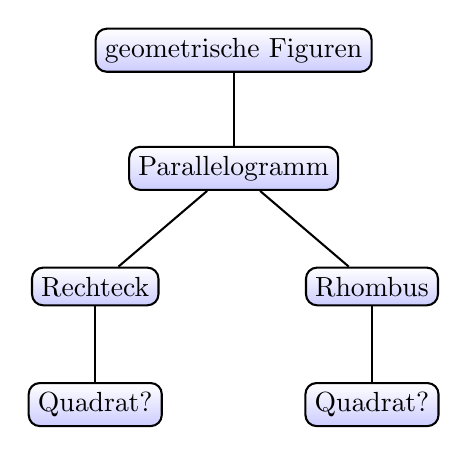
\begin{tikzpicture}[sibling distance=10em,
  every node/.style = {shape=rectangle, rounded corners,
    draw, align=center,
    top color=white, bottom color=blue!20}]]
  \node {geometrische Figuren}
    child { node {Parallelogramm} 
      child { node {Rechteck} 
      	child { node {Quadrat?}}}
      child { node {Rhombus} 
        child { node {Quadrat?} }}};
\end{tikzpicture}
		\caption{Einfachvererbung: Ist ein Quadrat ein Rechteck oder ein Rhomus?}
		\label{Abb:einfachvererbung}
	\end{center}
\end{figure}

\define{Eine Klasse:}\index{Klasse}
\begin{itemize}
	\item definiert einen abstrakten Datentyp (ADT)
	\item definiert ein Layout von Objekten / Instanzen dieses Typs (Instanzvariablen)
	\item definiert Datenfelder (Attribute) und Methoden (Funktionen)
	\item enthält Klassenvariablen (statische Variablen)
	\item enthält Konstruktoren (Default-Konstruktor ist immer da, hat 0 Parameter)
	\item enthält eventuell eine \code{main}-Methode
	\item kann nur aktiviert (aufgerufen) werden durch die JVM, falls die Klasse die \code{main}-Methode hat
\end{itemize}

\define{Ein Objekt / eine Instanz:}\index{Objekt}\index{Instanz}
\begin{itemize}
	\item repräsentiert eine Klasse / ist assoziiert zu einer Klasse
	\item muss erstellt werden durch einen Konstruktor
	\item enthält alle Instanzvariablen (entsprechend dem Layout der "Komponenten", die in der Klasse spezifiziert wurden)
	\item wird im dynamischen Speicher (heap) erstellt:
	Blockgröße wird bestimmt durch die Platzanforderungen von der Menge der Instanzvariablen
\end{itemize}

\subsection{Variablen und Typen}

\define{Typen:} verschiedene Kategorien:\index{Typen}
\begin{itemize}
	\item primitive (Daten-)Typen z.B. \code{boolean, int, long, double, ...}
	\item Referenztypen:
	\begin{itemize}
		\item Klassentypen z.B. \code{Boolean, Integer, Long, Double, ...}
		\item Interface-Typen
		\item Arraytypen
		\item Der \code{null}-Typ
	\end{itemize}
\end{itemize}

\define{Variablen:}\index{Variablen}
\begin{itemize}
	\item können jeden Typ haben (außer \code{null})
	\item Variablen von primitive Typen enthalten nur einen Wert von diesen primitiven Typ
	\item Referenzvariablen (Variablen von einem Referenztyp) enthalten eine Referenz\\ (Speicheradresse, Pointer) auf ein Objekt (eine Instanz) von einem kompatiblen Datentyp (welcher ein Subtyp der Variable sein muss) oder \code{null}
	\item sind entweder Datenfelder in einer Klasse, welche entweder 
	\begin{enumerate}[label=(\alph*)]
		\item \define{statische} Variablen (Klassenvariablen) einer Klasse
		\item \define{Instanzvariablen} (in jedem Objekt enthalten)
	\end{enumerate}
	oder \define{lokale} Variablen in Methoden (Stack-Variablen)
	\item \define{konstante} Variablen / \define{Konstanten} sind deklariert als \code{static final}
\end{itemize}

Speicherbereiche im Arbeitsspeicher:
\begin{itemize}
	\item statischer Speicher (Methodenaufruf-Speicher)
	\item dynamischer Speicher (Heap)
	\item Stapelspeicher (Runtime Stack)
\end{itemize}

\define{Methoden:}\index{Methoden}
\begin{itemize}
	\item sind entweder \define{Klassenmethoden} (\code{static}, sind wie klassische Funktionen) oder \define{Instanzmethoden} (werden auf der entsprechenden Instanz aufgerufen via einer Referenz zu dem Objekt)
	\item Methodenaufruf einer Klassenmethoden:\\ \code{Klasse.klassenmethode(param1,param2,...)}
	\item Methodenaufruf einer Instanzmethode: siehe Abbildung \ref{Abb:thisObj}\\ \code{referenzVariable.instanzmethode(param1,param2,...)}
	\item \define{Signatur:} Methodenname plus Liste der Parametertypen
	(Der Rückgabetyp (Return) ist auch wichtig, kann aber  in der Signaturdefinition weggelassen werden)
	\item \define{Overloading / Überladen:} 
	%\begin{itemize}
		%\item 
		es gibt mehrere Methoden mit demselben Methodennamen, aber unterschiedlichen Parameter-Typ-Listen (unterschiedliche Signatur)
	%\end{itemize}
	\item \define{Parameterübergabe}: immer "by value";
	bei Referenztypen wird die Referenz selbst übergeben
	\item \define{Overriding / Überschreiben:}
	erlaubt das Nutzen derselben Signatur in einer Unterklasse
	$\leadsto$ dynamisches / spätes Binden
\end{itemize}

\begin{figure}[H] % oder ht!
	\begin{center}
		% !TEX root = SCPROG.tex
% This work is licensed under the Creative Commons
% Attribution-NonCommercial-ShareAlike 4.0 International License. To view a copy
% of this license, visit http://creativecommons.org/licenses/by-nc-sa/4.0/ or
% send a letter to Creative Commons, PO Box 1866, Mountain View, CA 94042, USA.

\tikzset{every picture/.style={line width=0.75pt}} %set default line width to 0.75pt        

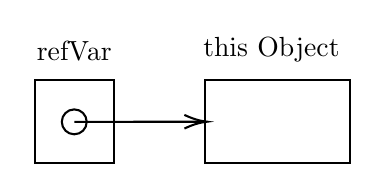
\begin{tikzpicture}[x=0.75pt,y=0.75pt,yscale=-1,xscale=1]
%uncomment if require: \path (0,300); %set diagram left start at 0, and has height of 300

%Shape: Rectangle [id:dp4673267372054163] 
\draw   (100,116) -- (138,116) -- (138,156) -- (100,156) -- cycle ;
%Shape: Rectangle [id:dp7209025887395226] 
\draw   (182,116) -- (252,116) -- (252,156) -- (182,156) -- cycle ;
%Shape: Circle [id:dp9831972127744683] 
\draw   (113,136) .. controls (113,132.69) and (115.69,130) .. (119,130) .. controls (122.31,130) and (125,132.69) .. (125,136) .. controls (125,139.31) and (122.31,142) .. (119,142) .. controls (115.69,142) and (113,139.31) .. (113,136) -- cycle ;
%Straight Lines [id:da3061374812316927] 
\draw    (119,136) -- (181,135.94) ;
\draw [shift={(183,135.93)}, rotate = 539.94] [color={rgb, 255:red, 0; green, 0; blue, 0 }  ][line width=0.75]    (10.93,-3.29) .. controls (6.95,-1.4) and (3.31,-0.3) .. (0,0) .. controls (3.31,0.3) and (6.95,1.4) .. (10.93,3.29)   ;


% Text Node
\draw (119,102) node  [align=left] {refVar};
% Text Node
\draw (214,101) node  [align=left] {this Object};


\end{tikzpicture}

		\caption{this Object: \code{this.instanzmethode(...)}}
		\label{Abb:thisObj}
	\end{center}
\end{figure}

\subsection{Literale (Konstanten von primitiven Datentypen)}
\begin{itemize}
	\item \code{int}: 32 Bit=4 Byte in Zweierkomplementdarstellung; Zahlenbereich:\\
	$-2^{31}=-2.147.483.648$ = \code{Integer.MAX\_VALUE} bis\\ $+2^{31}-1=2.147.483.647$ = \code{Integer.MIN\_VALUE}\\
	hexadezimale Repräsentation: \code{$\emptyset$x7ffffd}\\
	oktale Repräsentation: \code{$\emptyset$77$_{8}$=63$_{10}$}\\
	Unicode (16 Bit Zeichen): \code{$\setminus$u$\emptyset\emptyset$3f$_{16}$=63$_{10}$}
	\item \code{long:} 64 Bit = 8 Byte in Zweierkomplementdarstellung;
	Darstellung ähnlich wie \code{int}, mit einen postfix L:
	\code{longvar = 2147500000L;}
	(vergisst man hier das "L", so wird es nicht als long erkannt)
	Wertebereich: $\set{-2^{63},\ldots,+2^{63}-1}$ mit\\
	\code{Long.MAX\_VALUE, Long.MIN\_VALUE}
	Beispiel:
	\code{$\emptyset$x01fffaL}
	\item \code{byte} 8 Bit; \code{(byte) $\emptyset$x7e}
	\item \code{short} 16 Bit; \code{(short) 32767}\\
	Für \code{byte} und \code{short} gibt es \betone{keine} explizite Konstantennotation! (deshalb der Typecast)
	\item \code{float}: 32 Bit IEEE754 single precision floating-point\\
	\code{123.456F=0.123456e+3f=123456E-3F}\\
	Man kann die Null vor dem Komma weglassen und \code{.25} schreiben. 
	(Ob großes oder kleines \code{e} / \code{f} spielt keine Rolle)
	\item \code{double}: 64 Bit double precision;
	ähnlich wie \code{float} \betone{ohne} nachgestelltes (postfixed) Zeichen.
	Optional kann man das Zeichen "D" / "d" nachstellen.
	\code{Double.NaN}
	\item \code{char}: 16 Bit Unicodezeichen (ohne Vorzeichen!), z.B.\\ \code{'a','A',',','3',':', 'u$\setminus\emptyset\emptyset$47'}\\
	Escape-Sequenzen:
	\begin{itemize}
		\item \code{'$\setminus$n'} erzeugt Zeilenumbruch 
		\item \code{'$\setminus\setminus'$} erzeugt $\setminus$ (Backslash)
		\item \code{'$\setminus$''} erzeugt ' (single quote)
		\item \code{'$\setminus$\grqq{}'} erzeugt \grqq{} (double quote)
	\end{itemize}
	\item \code{boolean:} kann nur \code{true} oder \code{false}, \betone{keine} Typkonversion
\end{itemize}

\subsection{Typkonversionen (Casts / Casting)}
Implizite Typkonversionen:
\code{byte $\to$ short $\to$ int $\to$ long} und \code{char $\to$ int}
sowie \code{float $\to$ double}\\
Für die anderen Umwandlungen ist ein \betone{expliziter} Typecast notwendig.

\subsection{Binäre arithmetische Operationen}
Es gibt vier Hierarchie-Regeln:
\begin{enumerate}[label=(\arabic*)]
	\item Wenn mindestens ein Operand vom Typ \code{double} ist, dann ist das Ergebnis auch vom Type \code{double}.
	\item Wenn mindestens ein Operand vom Typ \code{float} ist, dann ist das Ergebnis auch vom Type \code{float}.
	\item Wenn mindestens ein Operand vom Typ \code{long} ist, dann ist das Ergebnis auch vom Type \code{long}.
	\item Alles andere liefert ein Ergebnis vom Typ \code{int}.
\end{enumerate}

\code{String}: automatische Umwandlung in \code{String}:\\
\code{str + primitive\_type\_value} bzw.  \code{primitive\_type\_value + str} \\
\code{str + reference\_type\_object} bzw. \code{reference\_type\_object + str}\\
Dies ruft automatisch die \code{toString()}-Methode auf dem Objekt auf.\\
Standardmäßig bekommt die hexadezimale Speicheradresse des Objektes, falls keine \code{toString()}-Methode deklariert ist.\\
Man sollte in jeder instanziierbaren Klasse eine \code{toString()}-Methode anlegen (\undefine{Overriding}).\nl
Der \define{instanceof-Operator} liefert \code{true} für alle Supertypen und den eigentlichen Typen.\\
\code{RefVar instanceof ClassName}, 
\code{x instanceof Object} ist immer \code{true}

\subsection{Vererbung (Inheritance)}
\code{[public] class MyClass \fbox{extends} Superclass \fbox{implements} IF1,IF2$\{\ldots\}$}

\subsection{Type-Konversion / Type Casting}
\begin{itemize}
	\item Implizite Type Casts sind für (viele) primitive Typen bereits vorhanden.
	\item Für \code{boolean} gibt es keine Typkonversion.
	\item \define{Upcasts} (Objekt als Objekt der Superklasse auffassen: Subtyp $\to$ Supertyp) funktioniert immer implizit.
	\begin{enumerate}[label=(\arabic*)]
		\item in Zuweisungen: \code{superVar = subExpr}.\\
		Der Cast \code{superVar = (SuperClass) subExpr} ist \betone{nicht} notwendig / optional.
		\item in Parameter-/Argument-Assoziationen: 
		Aufrufer übergibt (Referenz auf) ein Objekt des Subtypes (Subklasse) an einen formalen Parameter des Supertypes (Superklasse)
	\end{enumerate}
	\item \define{Downcast}: muss \betone{explizit} gemacht werden und beinhaltet einen (Compiler-\\generierten) Laufzeittest:\\
	\code{(TargetType) <Expression> // führt ggf. zu einer TypeCastException}
\end{itemize}

\subsection{\code{this} und \code{super}}
\begin{enumerate}[label=(\roman*)]
	\item In einer Instanzmethode (IM) oder einem Konstruktor\\
	\code{super} oder \code{this} referenzieren beide das sogenannte \define{this-Objekt}, auf welchem die Instanzmethode aufgerufen wurde (oder welches gerade "konstruiert" wird)\\
	\code{super.im(...)}
	\code{super.iv}
	\code{this.im(...)}
	\code{this.iv}

\begin{figure}[H] % oder ht!
	\begin{center}
		

\tikzset{every picture/.style={line width=0.75pt}} %set default line width to 0.75pt        

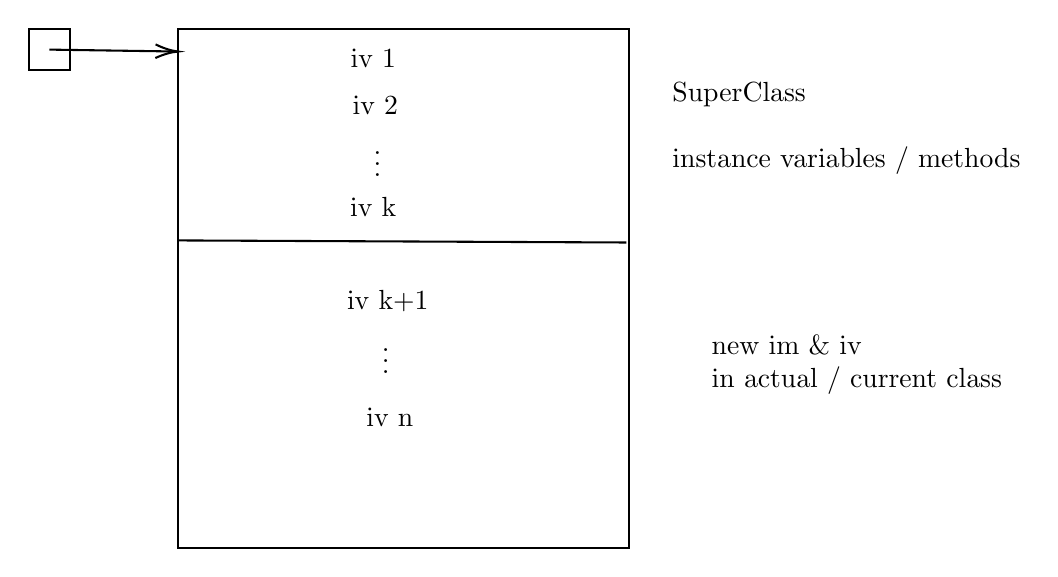
\begin{tikzpicture}[x=0.75pt,y=0.75pt,yscale=-1,xscale=1]
%uncomment if require: \path (0,300); %set diagram left start at 0, and has height of 300

%Shape: Rectangle [id:dp6411994266752609] 
\draw   (182,27.93) -- (399,27.93) -- (399,277.93) -- (182,277.93) -- cycle ;
%Shape: Square [id:dp3458024066933377] 
\draw   (110,28) -- (130,28) -- (130,48) -- (110,48) -- cycle ;
%Straight Lines [id:da4649876373916405] 
\draw    (120,38) -- (180,38.9) ;
\draw [shift={(182,38.93)}, rotate = 180.86] [color={rgb, 255:red, 0; green, 0; blue, 0 }  ][line width=0.75]    (10.93,-3.29) .. controls (6.95,-1.4) and (3.31,-0.3) .. (0,0) .. controls (3.31,0.3) and (6.95,1.4) .. (10.93,3.29)   ;

%Straight Lines [id:da2372718857026357] 
\draw    (182,129.93) -- (398,130.93) ;



% Text Node
\draw (276,42) node  [align=left] {iv 1};
% Text Node
\draw (504,76) node  [align=left] {SuperClass\\\\instance variables / methods};
% Text Node
\draw (509,190) node  [align=left] {new im \& iv\\in actual / current class};
% Text Node
\draw (277,65) node  [align=left] {iv 2};
% Text Node
\draw (276,114) node  [align=left] {iv k};
% Text Node
\draw (278,89) node   {$\vdots $};
% Text Node
\draw (283,159) node  [align=left] {iv k+1};
% Text Node
\draw (284,215) node  [align=left] {iv n};
% Text Node
\draw (282,184) node   {$\vdots $};


\end{tikzpicture}

		%\caption{Bildunterschrift}
		%\label{Abb:Titel}
	\end{center}
\end{figure}

Normalerweise ist \code{this.iv} semantisch äquivalent zu \code{iv} und \code{this.im(...)} semantisch äquivalent zu \code{im(...)}.
\newpage %TODO
\code{MyClass(int x)\{\\\tab this.x = x; // Die Ausnahme der Regel\\\}}\\
Andere Verwendung:\\
\code{ref = this;\\
return this; // \betone{nicht} in Konstruktoren!\\
methode(this);}
	\item In einem Konstruktor:\\
	\code{this(...); // ruft anderen Konstruktor in derselben Klasse auf\\
	super(...); // ruft anderen Konstruktor in der Mutterklasse auf}\\
	\href{https://stackoverflow.com/questions/586363/why-is-super-super-method-not-allowed-in-java}{Niemals \code{super.super(...)} schreiben!}
\end{enumerate}

\subsection{Overriding \& Dynamisches / Spätes Binden (während der Laufzeit)}
\begin{enumerate}[label=(\arabic*)]
	\item Compiler testet, ob Instanzmethodenaufruf möglich ist
	(in der Klasse der Referenzvariable)
	%\code{var.print()}
	\item Da Variablen polymorph sind, können sie Objekte jeder Unterklassen referenzieren (inklusive der Klasse selbst)
	\item \define{dynamisches / spätes Binden} beginnt also nach der korrekten Instanzmethode zu suchen, die auf dem Objekttyp / der Klasse aufgerufen werden soll.
	\index{dynamisches Binden}
	\index{spätes Binden|\see{dynamisches Binden}}
\end{enumerate}
$\implies$ Der Instanzmethodenaufruf funktioniert \betone{immer} (außer die Referenz ist \code{null})!

\subsection{Statisches Binden (während der Compilezeit)}
\index{statisches Binden}
\begin{itemize}
	\item alle Instanzmethoden in einer \code{final class} (verbietet Vererbung)
	\item alle Klassenmethoden (\code{static})
	\item alle Instanzmethoden, die mit \code{private} oder \code{final} (verbietet Overriding) deklariert wurden
\end{itemize}
$\implies$ Alle anderen Methoden nutzen dynamisches Binden während der Laufzeit!

\section{Anwendungsgebiete, Einschränkungen, Vor- und Nachteile}



